
\graphicspath{ {mainmatter/Roberts_2013/} }


\title*{2013: The Web Browser As Synthesizer And Interface}
\titlerunning{Web Browser As Synthesizer And Interface}


\author{Charles Roberts, Graham Wakefield, Matthew Wright}
\authorrunning{Roberts et al.}


%\institute{Charles Roberts \at School of Interactive Games \& Media, Rochester Institute of Technology\\ formerly Media Arts \& Technology Program, University of California at Santa Barbara, \email{charlie@charlie-roberts.com}
%\and Graham Wakefield \at School of Arts Media Performance \& Design York University \\ formerly Graduate School of Culture Technology, KAIST, \email{grrrwaaa@yorku.ca}}
%
%
\maketitle

\abstract*{Our research examines the use and potential of native web technologies for musical expression. We introduce two Java\-Script libraries towards this end: Gibberish.js, a heavily optimized audio DSP library, and Interface.js, a GUI toolkit that works with mouse, touch and motion events. Together these libraries provide a complete system for defining musical instruments that can be used in both desktop and mobile web browsers. Interface.js also enables control of remote synthesis applications via a server application that translates the socket protocol used by web interfaces into both MIDI and OSC messages.}

\section{Introduction}
Web technologies provide an incredible opportunity to present new musical interfaces to new audiences. Applications written in JavaScript and designed to run in the browser offer remarkable performance, mobile/desktop portability, and longevity due to standardization. As the web browser has matured, the tools available within it to create dynamic musical content have also progressed, and in the last two years realtime and low-level audio programming in the browser has become a reality. Given the browser's ubiquity on both desktop and mobile devices it is arguably the most widely distributed run-time in history, and is rapidly becoming a write once, run anywhere solution for musical interfaces. 

Additionally, web apps can now incorporate accelerometers, multitouch screens, gyroscopes, and fully integrated sound synthesis APIs, making web technologies suddenly very attractive for NIMEs. Our research stems from the desire to explore the affordances offered by NIMEs that are web apps and the belief that such instruments should be open and cross-platform. Ideally, a web-based musical interface should be able to run on desktop machines, laptops, and mobile devices regardless of the browser or operating system it is presented in. We believe the libraries described here are a significant step towards realizing this goal.

Our research is especially sympathetic to NIME developers wanting to take advantage of web technologies without having to learn the quirks and eccentricities of JavaScript, HTML and CSS simultaneously. We designed the syntax of Gibberish.js and Interface.js so that they can be utilized, both independently or in conjunction, almost entirely using JavaScript alone, requiring a bare minimum of HTML and absolutely no CSS (see Section~\ref{Roberts:sec:integrating}). The library downloads include template projects that enable programmers to safely ignore the HTML components and begin coding interfaces and signal processing in JavaScript immediately.

\section{Problems and Possibilities of the~Web Audio API}

In 2011 Google introduced the Web Audio API\footnote{\url{https://wiki.mozilla.org/Web_Audio_API}} and incorporated supporting libraries into its Chrome browser. The Web Audio API is an ambitious document; instead of merely defining a basic infrastructure for processing audio callbacks, the API  defines how audio graphs should be created and lists a wide variety of unit generators (``ugens'') that should be included in browsers as standard. These ugens are native pre-compiled %C++ 
objects that can be assembled into graphs and controlled by JavaScript. For better or for worse, the Mozilla Foundation had previously released a competing API (``Audio Data'') \cite{Humphrey:} that they integrated into the Firefox browser. This API also provided a well-defined mechanism for writing audio callbacks in JavaScript, however it provided no specifications for lower level, native, pre-compiled %C++ 
ugens to be standardly included in browsers. Fortunately, the Mozilla Foundation recently declared their intention to adopt the Web Audio API, suggesting that it will become the single standard for browser-based audio synthesis. In October of 2012, Apple rolled out iOS 6.0 to their phone and tablet devices and integrated the Web Audio API into mobile Safari; it seems likely to be adopted in other mobile platforms in the future, with promise of longevity through standardization. Our research supports both these APIs and automatically selects the correct one to use.

Although the Web Audio API comes with highly efficient ugens for common audio tasks such as convolution and FFT analysis, there are tradeoffs that accompany its usage. Most relate to the architectural decision to process blocks of at least 256 samples ($\approx 6$ ms) instead of performing single-sample processing. This places two notable restrictions on audio programming performed using the Web Audio API: lack of sample-accurate timing and inability to create feedback networks with short delays, which are necessary to important signal-processing applications including filter design and physical modeling. 

Fortunately, there is a workaround for these restrictions. The Web Audio API contains a specification for a JavaScript audio node that calculates output using JavaScript callbacks that can be defined at runtime. These guarantee sample-accurate timing and enable complex feedback networks, but at the expense of the efficiency that the native pre-compiled ugens provide. During our experiences developing \emph{Gibber} \cite{Roberts:2011a}, a live coding environment for the browser, we found that existing audio libraries (described in Section~\ref{Roberts:sec:RelatedWork}) built for this runtime JavaScript node were not efficient enough to realize the complex synthesis graphs we envisioned and thus began work on our own optimized library, \emph{Gibberish}.

\section{Gibberish: An Optimized JavaScript Audio Library}

The principal reason for JavaScript's excellent performance in the browser is the use of just-in-time (JIT) compilation: the virtual machine detects the most heavily used functions, path and type-specializations of the code as it runs, and replaces them with translations to native machine code. Although JIT compilation is making waves in the browser today, it can trace a long and diverse history to the earliest days of LISP\cite [p.7006]{Aycock:2003}. Now JIT compilers can approach and occasionally even beat the performance of statically compiled C code, though getting the best performance from a JIT compiler may call for very different coding habits than for a static compiler or interpreter. 

We began our research by looking at the performance bottlenecks associated with the JavaScript runtime and analyzing what could be done to ameliorate them. The most significant cost we found while working at audio rate in a dynamic runtime is the overhead of object lookup. In complex synthesis graphs, the simple task of resolving object addresses thousands of times per second (and potentially hundreds of thousands of times) levies a substantial cost. Gibberish minimizes this cost by ensuring that all data and functions used within the audio callback are defined and bound within the outer local scope (as ``upvalues''), avoiding the need for expensive indexing into externally referenced objects \cite{Herczeg:2009}.

\subsection{Code Generation}

Unfortunately, ensuring the locality of data and procedures for performance is not compatible with the flexibility to dynamically change the ugen graph, since adding or removing ugens implies changing the set of data and procedures that should be considered local to the audio callback. Our solution to this problem, inspired by  \cite{Wakefield:2012}, utilizes run-time code generation.

To optimize the audio callback the Gibberish code generation (``codegen'') engine translates the user-defined ugen graph created with object-oriented syntax into a single flat audio callback where all routing and modulation is resolved ahead of execution. This process is basically one of string manipulation. Each ugen is responsible for generating a fragment of code that invokes both its callback function and the callbacks of all ugens that feed into it. Since all inputs to ugens are resolved recursively, requesting the master output bus to perform code generation will effectively flatten the entire audio graph into a linear series of code fragments invoking ugen callbacks. These code fragments are then concatenated to form a string representing the master audio callback which is then dynamically evaluated into a callable function using JavaScript's \texttt{eval()} function.

As a simple example of the codegen algorithm in action, consider the following high-level programming syntax to create a frequency-modulated sine wave fed into a reverb that in turn feeds the default output bus:

{\small {\begin{verbatim}
modulator = new Gibberish.Sine( 4, 50 ); // freq, amp
carrier = new Gibberish.Sine({ amp : .1 });
carrier.frequency = add( 440, modulator );
reverb = new Gibberish.Reverb({ input:carrier });
reverb.connect();
\end{verbatim}}}

Traversing from the master output down through the graph, codegen will occur in the following order: \texttt{Bus > Reverb > Carrier > Add > Modulator}. The result is the following callback function, which will be called every sample:

{\small {\begin{verbatim}
function () {
  var v_16 = sine_5( 4, 50 ); 
  var v_15 = sine_8( 440 + v_16, 0.1 );
  var v_17 = reverb_11( v_15, 0.5, 0.55 );
  var v_4 = bus2_0( v_17, 1, 0 );
  return v_4;
}
\end{verbatim}}}

The \texttt{sine\_5}, \texttt{sine\_8}, \texttt{reverb\_11} and \texttt{bus2\_0} variables are all upvalues defined immediately outside the scope of the master audio callback and thus resolved inexpensively. These variables refer not to the ugens but to their signal processing functions (aka audio callbacks). The simplistic style of the generated code generally leads to improved run-time performance. For example, passing values by simple function arguments rather than using higher-level object properties and instance variables is ten percent faster in Google Chrome 26.\footnote{\url{http://jsperf.com/parameter-lookup-vs-instance-variables}}

Note that parametric properties of the ugens are translated as numeric literals (constants) in the generated code. By storing properties as compile-time constants, rather than using dynamic state, expensive calls to continuously index them are entirely avoided. However the implication, which may appear unusual, is that code generation must be invoked whenever a ugen property changes, in addition to when ugens are added or removed. In the above example, if we changed the frequency of our modulator sine wave from four to three Hertz, code generation would be retriggered. To reduce the cost of frequent regeneration, Gibberish caches and re-uses code for all ugens that have not changed. Whenever a ugen property is changed, that ugen is placed inside of a ``dirty'' array. During codegen each ugen inside the dirty array regenerates the code fragment that invokes its callback function; the code fragments for the rest of the ugens remain unaltered. Even if the callback is regenerated dozens or hundreds of times a second it still winds up being fairly efficient as only ugens with property changes invoke their codegen method; all ``clean'' ugens simply provide the last fragment they generated to be concatenated into the master callback. 

\subsection{Gibberish Ugens}
A variety of ugens come included with Gibberish, listed in Table~\ref{Roberts:tab:ugens}. In addition to standard low-level oscillators such as sine waves and noise generators, Gibberish also provides a number of higher-level synthesis objects that combine oscillators with filters and envelopes. These high-level objects provide a quick way to make interesting sounds using Gibberish and their source code also serves as guidance %provides templates 
for programmers interested in writing their own synth definitions.

It is fairly terse for users to add, redefine, or extend a Gibberish ugen at runtime. For example, here is the definition for the Noise ugen:

{\small {\begin{verbatim}
Gibberish.Noise = function() {
  this.name = 'noise';
  this.properties = { amp:1 };
  this.callback = function( amp ) {
    return ( Math.random() * 2 - 1  ) * amp;
  };
  this.init();
}
Gibberish.Noise.prototype = Gibberish.Ugen;
\end{verbatim}}}

The \texttt{init()} method is inherited from the Ugen prototype and sets up code generation routines for the ugen in addition to performing other initialization tasks. The \emph{properties} dictionary in the ugen definition identifies properties that are used in the ugen's callback method signature, and specifies their default values. When code generation occurs, the order that individual properties are enumerated in this dictionary defines their order in the ugen's callback method signature.

\begin{table}[t]
\centering
\caption{Gibberish Ugens by Type}
\begin{tabular}[hb]{l | l}
\hline
Oscillators & \begin{minipage}[t]{0.75\columnwidth} Sine, Triangle, Square, Saw, Bandlimited Saw, Bandlimited PWM / Square, Noise \end{minipage} \\
\rule{0pt}{3ex}
Effects & \begin{minipage}[t]{0.75\columnwidth} Waveshapers, Delay, Decimator, Ring Modulation, Flanger, Vibrato, Chorus, Reverb, Granulator, Buffer Shuffler / Stutterer. \end{minipage} \\
\rule{0pt}{3ex}
Filters & \begin{minipage}[t]{0.75\columnwidth} Biquad, State Variable, 24db Ladder, One~Pole \end{minipage} \\
\rule{0pt}{3ex}
Synths & \begin{minipage}[t]{0.75\columnwidth} Synth (oscillator + envelope), Synth2 (oscillator + filter + envelope), FM (2 operator), Monosynth (3 oscillator + envelope + filter) \end{minipage} \\
\rule{0pt}{3ex}
Math & \begin{minipage}[t]{0.75\columnwidth} Add, Subtract, Multiply, Divide, Absolute Value, Square Root, Pow \end{minipage} \\
\rule{0pt}{3ex}
Misc & \begin{minipage}[t]{0.75\columnwidth} Sampler (record \& playback), Envelope Follower, Single Sample Delay, Attack/Decay Envelope, Line/Ramp envelope, ADSR Envelope, Karplus-Strong, Bus \end{minipage} \\
\end{tabular}
\label{Roberts:tab:ugens}
\end{table}

\subsection{(Single Sample) Feedback}
Allowing single sample feedback is a benefit of processing on a per-sample basis instead of processing buffers. It can be achieved in Gibberish using the Single Sample Delay (SSD) ugen. This ugen samples and stores the output of an input ugen at the end of each callback execution and then makes that sample available for the next execution. Below is a simple feedback example with a filter feeding into itself:

{\small {\begin{verbatim}
pwm = new Gibberish.PWM();
ssd = new Gibberish.SingleSampleDelay();

filter = new Gibberish.Filter24({
  input: add( pwm, ssd ),
}).connect();
ssd.input = filter;
\end{verbatim}}}

In the generated callback below note that there are two functions for the SSD ugen. One records an input sample while the other outputs the previously recorded sample.

{\small {\begin{verbatim}
function () {
  var v_7 = single_sample_delay_3();
  var v_5 = pwm_2(440, 0.15, 0.5);
  var v_6 = filter24_1(v_5 + v_7, 0.1, 3, true);
  var v_4 = bus2_0(v_6, 1, 0);
  single_sample_delay_8(v_6,1);
  return v_4;
} 
\end{verbatim}}}


\subsection{Scheduling and Sequencing}
\label{Roberts:sec:scheduling}

Although the JavaScript runtime includes its own methods for scheduling events, there is no guarantee about the accuracy of the time used by this scheduler. Accordingly, the only way to ensure accurate timing is to perform event scheduling from within the audio sample loop. This in turn means that any JavaScript DSP library that performs automatic graph management and callback creation (as Gibberish.js does) must also provide a mechanism for event timing that is synchronized to the audio sample loop. Gibberish.js contains a \texttt{Sequencer} object that can be used to sequence changes to property values, calls to methods, or execution of named or anonymous functions at user-defined rates with sample-accurate timing.

The syntax for a sequencer uses a simple target/key mechanism. A sequencer's \emph{target} specifies the ugen (or any other JavaScript object---scheduling is not limited to controlling ugens) that the sequencer will control. The \emph{key} specifies the name of a property that should be set or a method that should be called by the sequencer. The \emph{values} array defines the values that are passed to object methods or assigned to object properties, while the \emph{durations} array controls how often the sequencer fires off events. By default time is specified in samples, but convenience methods are provided for converting milliseconds, seconds, and beats to samples. Thus, the following sequences a \texttt{FMSynth} looping through three pitches and alternating between half a second and a quarter second duration:

{\small {\begin{verbatim}
a = new Gibberish.FMSynth().connect();

b = new Gibberish.Sequencer({
  target: a, key: 'note,'
  values: [ 440, 880, 660 ],
  durations: [ seconds(.5), seconds(.25) ],
}).start();
\end{verbatim}}}

Musicians may also want to attach more than one property change or method call to each firing of a sequencer object, for example,  changing an oscillator's amplitude whenever its frequency changes. To accommodate this the Sequencer object can accept a \emph{keysAndValues} dictionary that can feature multiple key/value pairs to be sequenced.

{\small {\begin{verbatim}
a = new Gibberish.Sine().connect();

b = new Gibberish.Sequencer({
  target: a,
  durations: [ beats(2), beats(1), beats(1) ],
  keysAndValues:{
    frequency: [ 440, 880, 660 ],
    amp: [ .5, .25 ],
}).start();
\end{verbatim}}}

This keysAndValues syntax has similarities to SuperCollider's \emph{Pbind} object \cite{Kuivila:2011}, which also enables the sequencing of multiple parameters using the same timing. 

When a values array contains a function, the Sequencer will simply invoke it (with no arguments) to determine the value it should use; this enables the sequencer to schedule arbitrary behavior such as randomly picking elements from an array.  Functions within a sequencer's \texttt{values} array will still be called even if the Sequencer has no specified target, supporting sample-accurate sequencing of any arbitrary JavaScript function (for example, to synchronize state changes of multiple ugens).

\section{Interface.js}

Interface.js provides a solution for quickly creating GUIs using JavaScript that work equally well with both mouse and touch interaction paradigms. The output of these GUI widgets can control other JavaScript objects (such as Gibberish ugens) and/or be converted to MIDI or OSC \cite{Wright:2005} messages via a small server program that is included in the Interface.js download. This means Interface.js can be used both to control programs running in the browser and also to control external programs such as digital audio workstations.

Interface.js includes a useful array of visual widgets for audiovisual control, including \texttt{Button}, \texttt{MultiButton}, \texttt{Slider}, \texttt{MultiSlider}, \texttt{RangeSlider}, \texttt{Knob}, \texttt{XY} (multitouch, with physics),  \texttt{Crossfader}, \texttt{Menu}, \texttt{Label}, and \texttt{TextField}.

Interface.js also provides unified access to accelerometer readings and the orientation of the device. These motion-based sensors work on most mobile devices as well as the desktop version of Google Chrome.

\subsection{Event Handling in Interface.js}

Interface.js binds widgets to object functions and values using a target / key syntax similar to the Gibberish sequencer (see Section~\ref{Roberts:sec:scheduling}). A widget's \emph{target} specifies an object and the \emph{key} specifies a property or method to be manipulated. What happens when a widget value changes depends on what the key refers to: object properties are \emph{set} to the new widget value, while object methods are \emph{invoked} with the widget value as the first argument. Widgets providing multiple dimensions of control (e.g., XY, accelerometer...) are configured with arrays of targets and keys with one target and one key for each dimension of control.

Users can also register custom event handlers to create more complex interactions than direct mappings between widgets and property values. Although most browsers only deal with either touch or mouse events, Interface.js provides another type of event handler, \emph{touchmouse events}, that respond to both forms of input. The specific events are:

\begin{itemize}
\item \texttt{ontouchmousedown}: when a mouse press begins or a finger first touches the screen
\item \texttt{ontouchmousemove}:  when a mouse or finger moves after a start event
\item \texttt{ontouchmouseup}:  when a mouse press ends or a finger is removed from the screen
\end{itemize}

There is also a fourth event handler, \texttt{onvaluechange}, that is called every time the value of a widget changes, regardless of whether the widget changes by touch, the mouse, or by motion. Procedurally changing a widget's value (perhaps due to the output of another widget) will also trigger this event. Although the touchmouse and onvaluechange event handlers provide a unified interface for dealing with all events, users are free to register for dedicated mouse or touch events if they want to change how interactivity functions across different modalities.

\subsection{Interface Layout And Appearance}
The main container unit of Interface.js is the \emph{Panel} widget. Panel wraps an instance of the HTML \emph{canvas} element, a 2D drawing surface with hardware graphics acceleration support in all current desktop browsers and most current mobile browsers. Panel's constructor allows users to specify a HTML element for the canvas tag to be placed inside, allowing multiple panels to be placed at different points in a HTML page.  If no container HTML element is provided, Interface.js will automatically create a canvas element that fills the entire window and attach it to the HTML page; this minimizes the HTML needed to create a GUI.

Widget sizes can be integer pixel values or float values giving the size relative to the widget's enclosing Panel. For example, consider placing a Slider inside a $500\times500$ pixel Panel. If the Slider's \texttt{x} value is .5, then its leftmost edge will be inset 250 pixels at the horizontal center of the panel. If the Slider's width is also .5, it will extend 250 pixels from the horizontal center to the rightmost edge of the Panel. Using relative layouts enables users to define interfaces without having to worry about varying window sizes or the screen sizes of different devices. An exception to this would be creating an interface for a large screen with a large number of widgets and then trying to view the same interface on a smartphone; in this case the widgets, although positioned and sized correctly, would be too small to use for accurate interaction.

In lieu of using CSS to specify colors, Interface.js instead allows them to be defined programmatically using JavaScript. By default, a widget uses the background, fill and stroke properties assigned its container Panel object. Thus, by default, all widgets in the same Panel use the same set of colors. Changing the color properties of a Panel object immediately changes the colors of its child widgets. If color properties for an individual widget are explicitly set their values will override the Panel's default values.

\subsection{Preset Management}
Interface.js allows programmers to easily store the values of widgets in an interface for instant recall. A call to the method \texttt{Interface.Preset.save('preset name')} will serialize the values of all widgets in the current interface and convert the resulting object to a string that can be stored using the HTML \texttt{localStorage} object. 

\texttt{Interface.Preset.load('preset name')} loads a preset. When a preset is loaded every widget sends out its target / key message (if so defined) and executes its \texttt{onvaluechange} event handler if the new value differs from the widget's current value.

\subsection{Networked Control}

\begin{figure}[t]
    \centering
		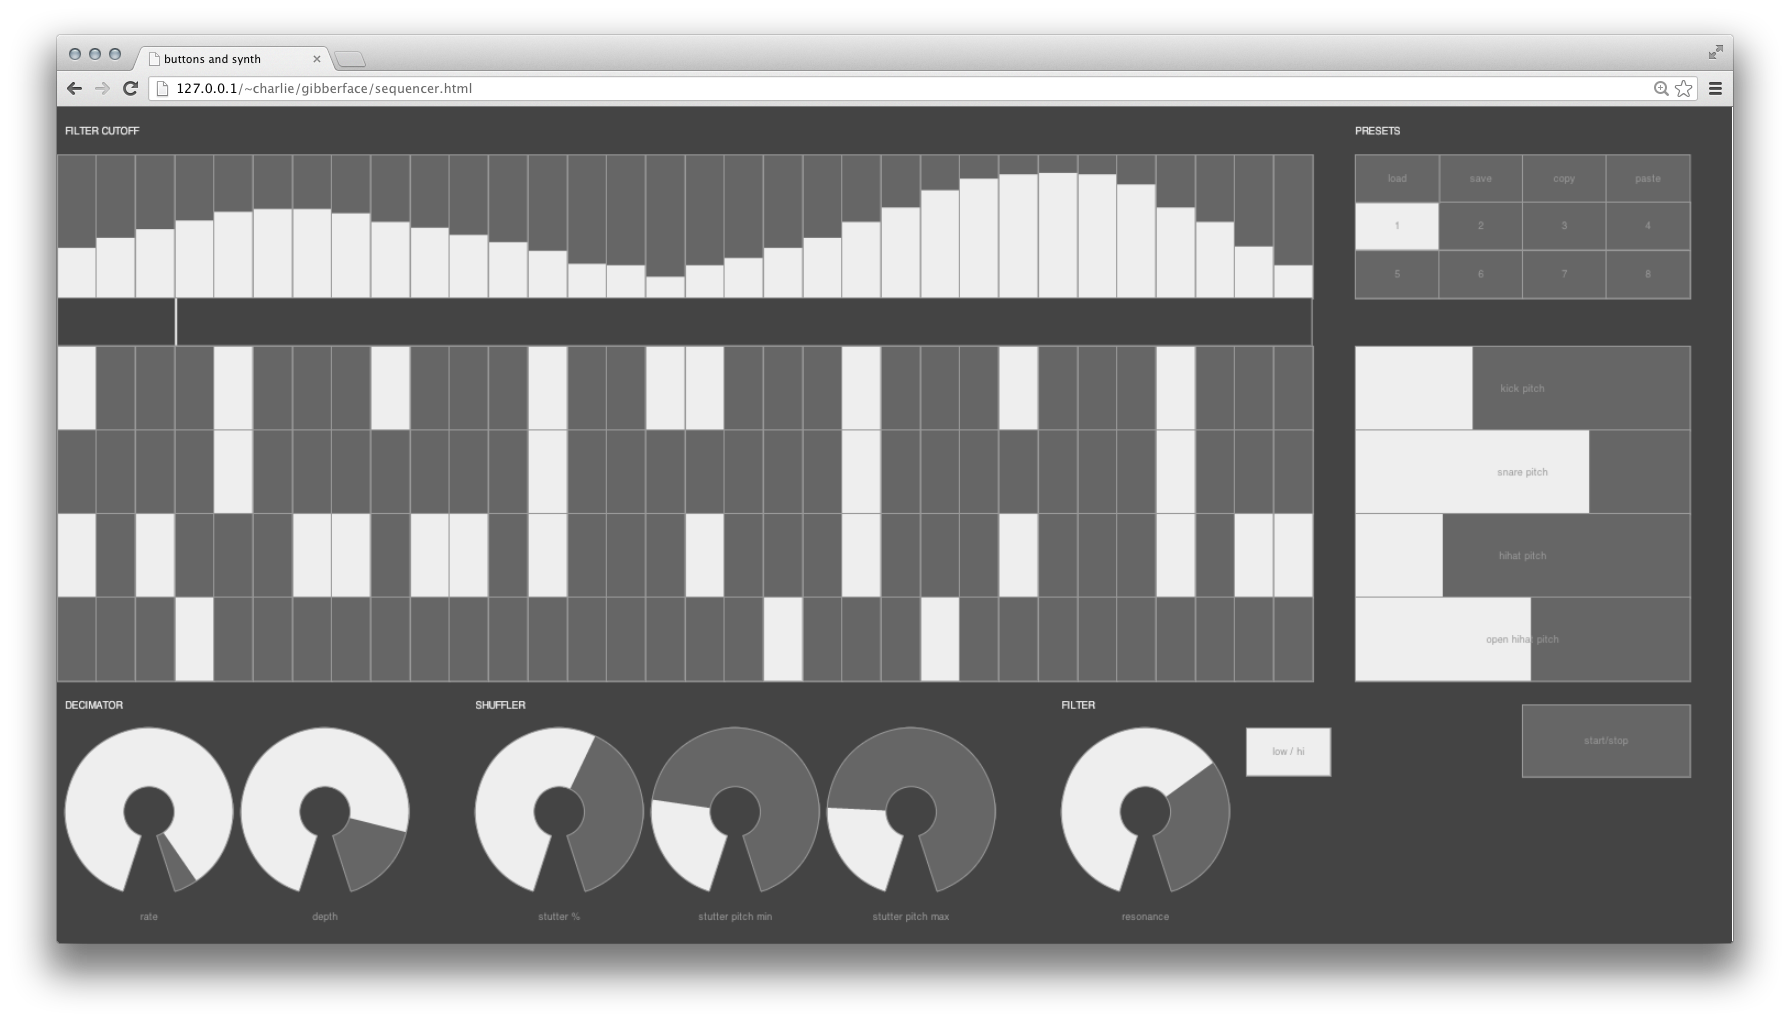
\includegraphics[width=\textwidth]{screenshot}
	\caption{A drum sequencer with four tracks of 32nd notes and controls for various effects}
\label{Roberts:fig:drumsequencer}
\end{figure}

As an alternative to controlling Web Audio synthesis graphs or other JavaScript objects, Interface.js can also transmit output over a network via the WebSocket API in order to control remote applications. The WebSocket API sends messages over TCP but features a handshake mechanism relying on the HTTP protocol. Since most musical applications do not understand the WebSocket API, it becomes necessary to translate messages received from a WebSocket to a more appropriate musical messaging protocol, such as OSC or MIDI.

Although there have been previous efforts creating servers that translate WebSocket data into OSC or MIDI messages, we believe our solution is uniquely efficient. Instead of simply creating a server that waits for incoming WebSocket messages and then forwards them using OSC or MIDI, we have included a HTTP server that serves interface files to client devices. After launching our server application, any user directing a client browser to the server's IP address (on port 8080) will receive an HTML page listing available interfaces stored in the server's default storage directory. When a user selects an interface, it is downloaded to their browser and a WebSocket connection is automatically created linking their client device to the server; in other words, the computer that serves Interface.js pages is automatically also the recipient of the WebSocket messages generated by such interfaces. WebSocket messages sent from the interface are translated into OSC or MIDI messages based on the contents of individual interface files.  

A distinct advantage of this system is that programmers do not need to think about establishing socket connections when developing their interfaces; there are no hardcoded IP addresses and no auto-discovery protocols needed. The IP address and port is entered once when first accessing the server; after that the location can be bookmarked for easy access. Individual interfaces can also be bookmarked; in this case the WebSocket connection is established as soon as the interface bookmark is selected. On mobile devices these bookmarks can be represented by icons on user's home screens; simply tapping such icons fetches the interface and immediately opens the appropriate connection.

In order to indicate that a widget's output should be sent over the network, a target of Interface.OSC or Interface.MIDI is assigned. For widgets that target Interface.OSC, the key property then represents the address the message will be sent to. For widgets targeting Interface.MIDI, the key is an array containing the message type, channel, and number (if it is a three-byte MIDI message) for the output MIDI message. Multiple devices (and thus users) can load interfaces from the server and send messages for translation and forwarding simultaneously.

\section{Integrating Interface.js and Gibberish.js}
\label{Roberts:sec:integrating}

There a few simple steps in order to use Interface.js and Gibberish.js together to make a musical interface. Starting with an HTML document containing the bare minimum necessary tags (\texttt{<html>, <head> \& <body>}), add two \texttt{<script>} tags to import the Gibberish and Interface Javascript files. A third \texttt{<script>} tag inside the body element contains all user code to create the interface and/or audio graph. The following complete sample interface file creates a sine tone controlled by two sliders:

{\small 
\begin{verbatim}
<html>
<head>
  <script src="interface.js"></script>
  <script src="gibberish_2.0.min.js"></script>
</head>

<body>
  <script>
  Gibberish.init();
  sine  = new Gibberish.Sine().connect();
  var panel = new Interface.Panel();
  
  sliderFrequency = new Interface.Slider({
    target:sine, key:'frequency,'
    min:150, max:1000,
    \label{Roberts::'freq,' bounds:[ 0,0,.3,1 ],
  });
    
  sliderAmp = new Interface.Slider({
    target:sine, key:'amp,'
    \label{Roberts::'amp,' bounds:[ .3,0,.3,1 ],
  });
    
  panel.add( sliderFrequency, sliderAmp );
  </script>
</body>
</html>
\end{verbatim}
}

% Nuff said. Awesome.

\section{Related Work}
\label{Roberts:sec:RelatedWork}

There are a growing number of options for writing synthesis algorithms in JavaScript in the browser. Audiolib.js\footnote{\url{http://audiolibjs.org}} was one of the first significant JavaScript audio libraries written and still provides an excellent array of synthesis options. It was our original choice for Gibber; we abandoned it only after discovering that code generation often leads to more efficient performance. Audiolib.js performs no graph management leaving programmers to implement their own audio graphs.

Other libraries take vastly different approaches in terms of the APIs they offer programmers. For example, Flocking\footnote{\url{https://github.com/colinbdclark/Flocking}} enables users to define new ugens declaratively using JavaScript Object Notation (JSON), while Timbre.js\footnote{\url{https://mohayonao.github.io/timbre.js/}} is a very impressive library that enables users to compose ugens in a functional syntax inspired by jQuery, a JavaScript library for HTML manipulation. In addition to its extensive use of code generation techniques, Gibberish.js differentiates itself from these other libraries by containing several more complex pre-composed synthesis ugens. For example, Gibberish offers a polyphonic, enveloped two-op FM synthesis ugen; to our knowledge no other JavaScript libraries offer FM synthesis engines with easy control over carrier to modulation ratios and index properties. Another example of a complex pre-composed ugen is the Gibberish Monosynth, a three-oscillator bandlimited synthesizer with an envelope, 24db resonant filter, and independent tuning and waveshape controls for each oscillator. By including complex ugens we allow programmers to begin creating music with rich sound sources immediately.

Another solution for web based synthesis is JSyn \cite{Burk:1998}, a Java synthesis library originating over a decade ago. Unfortunately many browsers do not support Java by default, and many do not support it at all (including Safari on iOS).

Although there are many other HTML / JavaScript interface libraries, very few understand both touch and mouse modalities and almost none are catered towards the needs of musicians and live performers. A extension to jQuery named Kontrol\footnote{\url{http://anthonyterrien.com/kontrol/}} provides well-engineered virtual knobs and slider banks that respond to both touch and mouse events. However, there is no support for control areas tracking multiple touches across a single rectangle; in our opinion this is one of the most useful widgets for performance on touchscreen devices. The Interface.js XY widget tracks up to 11 touches simultaneously and also features a built-in physics engine, inspired by the JazzMutant Lemur.\footnote{\url{http://www.jazzmutant.com/lemur_overview.php}} In addition to providing only three widgets, the Kontrol library also requires knowledge of HTML and of the jQuery library. In general the library is targeted towards existing web developers while Interface.js attempts to shield programmers from HTML and CSS as much as possible.

The massMobile project  \cite{Weitzner:2012} allows audience participation in performances through web interfaces on mobile devices that output to a database that can be read by Max/MSP externals. It is interesting to note that this project started with dedicated client applications for iOS and Android before switching to use web technologies in order to become usable on a wider variety of devices. A notable precursor to the massMobile project was the composition Telemusic \#1, by Randall Bradley, Steve Young and John Young \cite{Young:2001}. In this piece, users accessed a website with an embedded Flash animation that communicated with a Java applet running in the same page; this Java applet then forwarded information to a remote instance of Max/MSP.

\section{Conclusions and Future Work}
Both Gibberish.js and Interface.js are open-source and available for download on GitHub.\footnote{\url{https://github.com/charlieroberts/Gibberish} and \url{https://github.com/charlieroberts/interface.js}} A separate code repository, \emph{Gibberface},\footnote{\url{https://github.com/charlieroberts/gibberface}} contains examples integrating both libraries, ranging from the simple (as in Section~\ref{Roberts:sec:integrating} above) to more complex interfaces and audio graphs such as the drum sequencer shown in Figure~\ref{Roberts:fig:drumsequencer}.

Part of the inspiration for Interface.js came from our work on the mobile application \emph{Control} \cite{Wright:2005}. Control allows users to create interfaces for controlling remote applications with web technologies but also provides access to device features that are not exposed in browsers, such as the ability to send and receive OSC and MIDI. Advances in JavaScript APIs have exposed more and more functionality to mobile browsers' JavaScript runtime; gyro and compass sensors are two examples of sensors that were not accessible in the browser two years ago that now have established APIs. There are still a number of sensors commonly available on mobile devices that are inaccessible to JavaScript or impractical to process efficiently. As one example, detecting the surface diameter of individual touches can be used to create a crude yet surprisingly musical ``aftertouch'' signal that is not possible to read using browser APIs alone. As more APIs providing access to sensors become available in mobile browsers we will update Interface.js to take advantage of them.

In Gibberish there is a particular need for more analysis ugens beyond the simple envelope follower that currently exists. Gibberish has already been integrated into the live coding environment Gibber and numerous group and solo performances have been conducted using it as the synthesis engine. The first author has recently performed in concert using an instrument created with Gibberish.js and Interface.js on a tablet device; a modified version of this interface, which uses multitouch tracking to control bandlimited pulsewidth modulation oscillators, is included in the Gibberface repository.


\section*{Author Commentary: Reflections on Synthesis and Instrument Design for the Browser}

\paragraph{Charlie Roberts, Graham Wakefield, and Matthew Wright} 
 
In 2013, fast JavaScript implementations were proliferating beyond desktop browsers to mobile devices, while new developments in browser technology were making plugin­free implementations of real­time audio synthesis feasible. Our article presented a portable, flexible, and optimized audio library, Gibberish.js, coupled with a library to bring together device capabilities and common user interface elements, ​Interface.js, to explore browser­based NIMEs within the capabilities of JavaScript running entirely inside a web browser.
 
Browser­based audio synthesis has since seen significant advances, including a standardized API (the WebAudio API, or WAAPI​)\footnote{\url{http://www.w3.org/TR/webaudio/}} for creating audio graphs from a fixed library of pre­compiled unit generators that function across all modern web browsers. A number of excellent libraries have since been written using the nodes provided by the WAAPI  \cite{Choi:2013,Mann:2015}. Although Google had begun work on this API when we began our research, it had yet to be adopted by other major browsers; using audio synthesis code written in JavaScript was the most portable solution at the time. Instead of processing unit generator nodes in blocks, Gibberish.js dynamically generates optimized JavaScript which processes the graph sample by sample, as the paper details. This enables important categories of synthesis and signal processing such as feedback FM, customized filter architectures, certain physical models, and audio­rate modulation of scheduling. Pre­compiled unit generators can guarantee lower latencies and higher throughput, but only at the price of this flexibility. As of Fall 2015 still no other JavaScript audio synthesis libraries capitalize on per­sample processing techniques to the best of our knowledge. With upcoming updates to JavaScript engines and the WebAudio API the per­sample approach taken by Gibberish.js may become more appealing. Latencies will be reduced via WebWorkers​\footnote{\url{http://webaudio.github.io/web-audio-api/}} that perform audio signal processing written in JavaScript in a dedicated thread, free of pauses caused by UI interaction and networking. Efficiency may be increased by targeting code generation to lower levels via WebAssembly.​\footnote{\url{https://github.com/WebAssembly/design/blob/master/HighLevelGoals.md}} As options for running audio engines in the browser diversify, we predict the need for end­user languages that will use meta­programming to match user requirements to target language and engine capabilities, whether block­based WAAPI nodes, WebWorkers, WebAssembly, or otherwise. Researchers porting Csound to the browser have already made progress in this area, comparing implementations of Csound using WebAssembly to a PNaCl plugin in Google Chrome  \cite{Lazzarini:2014}, and we plan to continue exploring these ideas in Gibberish.js.
 
The current version of Gibberish.js has served as an important foundation for the creative coding environment ​ Gibber, which has seen international use in a variety of performative and educational contexts. We are also happy to see increasing use of Gibber and Gibberish.js by other researchers. For example, Taylor et al. used Gibberish.js to create a live coding environment, ​\emph{Braid}, for digital musical instrument design  \cite{Taylor:2015}, while Lee et al. used it to explore the applications of recording and playing back text entry for live coding and live writing  \cite{Lee:2015}. We look forward to continuing the improvement of both Gibber and Gibberish.js with help and critique from the NIME community.
 
The domain of plug­in free, browser­based NIMEs is still nascent. Our contribution addressed a particular problem (cross­browser, per­sample signal processing) during early days of architectural exploration; years later, critical components of a standardized audio engine for the browser remain in flux. We hope our research can help inform future synthesis libraries as the design, standardization and implementation of audio architectures in the browser continue to be refined.


\section*{Expert Commentary: The potential synthesizer in your pocket}

\paragraph{Abram Hindle} 

Before the browsers clearly adopted HTML5, writing a coherent user interface usually required platform specific code. Writing an app for a mobile phone required addressing each platform individually, and multimedia support was even more difficult. Yet a new breed of programmer was on the horizon, the client-side web programmer who were suddenly capable of writing multi-media rich portable graphical user interfaces (GUIs) that could run on desktops and mobile devices---but only if the technology could be adopted by enough end-users. 2012 was that time, with increased smartphone penetration combined with better mobile browser support 2012 ushered in web-GUIs that were mobile compatible.

Around the same time in 2012, as described by  \cite{Roberts:2013}, the browser community finally started to come together around a coherent WebAudio specification\footnote{\url{http://www.w3.org/2011/audio/}}, a standard where a couple of extra lines Javascript could patch over any incompatibilities. In fact WebAudio was even working well within many smart-phone browsers, such as Mobile Safari and Firefox Mobile, by the start of 2013.\footnote{\url{http://caniuse.com/\#feat=audio-api}} Thus the developments of 2012 enabled the mass adoption of HTML5 technologies by the majority of consumers.

The NIME community take-away is that HTML5 lets us deploy a synthesizer on every desk and in every smartphone pocket. Mass adoption combined with portability makes any HTML5-enabled device a potential synthesizer or NIME. This observation was not lost on the 2013 NIME community who in the same year published 4 or more web-GUI/WebAudio papers at the same conference. But there was 1 big glaring problem: your synthesizer is programmed in a flexible yet interpreted language, with a very limited audio API that makes lots of delays and filters quite difficult to implement efficiently or at all. Thus both developer productivity and run-time performance were at stake.

What Roberts et al. provide is a library of ugens, synths and temporal control structures leveraging the \texttt{ScriptProcessor node}, which affords the authoring of sample-level signal processing algorithms in JavaScript. This module lets one write raw samples to the soundcard's buffer, thus if you needed single sample accuracy you would have to do it here---which is exactly what they implemented. They did a lot of the heavy lifting of mixing and scheduling audio that addressed certain performance issues and certain missing \texttt{ugens} but it still didn't address the generally poor performance of Javascript and many WebAudio implementations.

 \cite{Roberts:2013} addressed some of Javascript's inefficiencies for signal processing by taking advantage of the language's flexibility. Modern JavaScript engines use just-in-time (JIT) compilation engines to compile well-written JavaScript into lower-level representations with improved efficiency. As JavaScript can also evaluate code contained within strings,  \cite{Roberts:2013} used their own code-generation engine to dynamically generate JIT-friendly Javascript from terse specifications.

In my opinion this work seemed immediately valuable to the NIME community for 3 reasons and is still relevant and valuable: 1) the software is still actively maintained, it works, and you can deploy it on just about anything; 2)  \cite{Roberts:2013} have provided a clear framework and methodology for achieving similar successful results with WebAudio; 3) WebAudio is here to stay, Web GUIs are supplanting classic native GUIs as the functionality of HTML5 implementations improve.

The work has limitations that software tends to face, it was somewhat of a work in progress at the time, attempting to deal with the ever changing WebAudio specifications and implementations available at the time. In 2015 the WebAudio specification and capabilities continue to evolve, this violates Roberts et al.'s claim that WebAudio code is a ``write once, run anywhere solution.'' For instance the WebAudio specification is deprecating the ScriptProcessorNode for the AudioWorkerNode. Yet the work is ever more prescient than ever as the adoption and support of HTML5 interfaces and HTML5 multimedia is more than ever before.

Gibber is still being updated to this very day and so is the WebAudio specification. I encourage anyone who takes part in low-level WebAudio development to take part in the W3C's web audio working group. This group is well meaning but they do not necessarily share the same problems or have the same needs and experiences as many of those in the NIME community; your feedback and experience is invaluable to a working group like this. Thus Gibber still fills many important niches that the W3C WebAudio specification has yet to fill.
